\documentclass[class=NCU_thesis, crop=false]{standalone}
\begin{document}

\chapter{研究方法}

\section{系統架構} \label{ch3-st-system-structure}
\fig[1][fig:fig-ch3-system-structure-overview][!hbt]{ch3/fig-system-structure-overview.png}
[系統架構圖][系統架構圖]

\cref{fig:fig-ch3-system-structure-overview} (A)
為本系統的整體架構,此系統可分為離線處理與線上處理兩個階段,
離線處理階段會將混合音源分離成參考音訊與伴奏音訊作為線上處理階段的資料,
線上處理階段接收演奏者的即時串流音訊,並結合參考音訊來計算目前演奏者的樂曲位置,
並根據樂曲位置輸出對應的伴奏音訊。
請注意本研究將小提琴與鋼琴之混合音訊作為主要資料,
並專注在當演奏者樂器為小提琴或鋼琴的情況下來使用本系統。

\cref{fig:fig-ch3-system-structure-overview} (B)
為音源分離模組的細部架構,
採用深度學習模型將混合音訊中的目標音源分離出來。
此模組包含了小提琴(參考音訊)音源分離模型與鋼琴(伴奏音訊)音源分離模型,
另外在訓練階段,本研究設計了一種簡單的頻帶切割估計方法提升模型的分離效果。
關於模型架構、頻帶切割估計方法會在\ref{ch3-st-mss-module}節做討論。

\cref{fig:fig-ch3-system-structure-overview} (C)
為音樂追蹤模組的細部架構,
此模組使用Python 3.9開發,
我們使用multiprocessing package~\cite{python2024multiprocessing}實現平行化處理,
串流音訊使用pyaudio package~\cite{python2024pyaudio}接收處理,
達到即時追蹤與伴奏的效果。
此模組包含四個元件,
分別為資料管理者(Data Manager)、音樂偵測器(Music Detector)、
粗略位置估計器(Rough Position Estimator)與決策決定者(Decision Maker)。
資料管理者管理所有音訊的資料與特徵、
音樂偵測器即時偵測音樂是否開始、
粗略位置估計器估計整段參考音訊中可能的伴奏時間位置,提供決策決定者更多選擇、
決策決定者即時計算目前輸出位置並決定最後的輸出位置,
關於元件詳細的設計與改動會在\ref{ch3-st-music-tracking-module}節做討論。

\pagebreak

\section{音源分離模組} \label{ch3-st-mss-module}

\subsection{Band-Split RNN} \label{ch3-subst-band-split-RNN}
Band-Split RNN(BSRNN)~\cite{Luo_Yi2022MusicSourceSeparation}
由Luo Yi等人於2022年提出,是一種專門為高取樣率訊號所設計的時頻域音源分離模型。
BSRNN將輸入的頻譜圖$X\in \mathbb{C} ^{F\times T}$
根據自定義的頻帶切割點$G = (G_1, G_2, \dots G_i), \sum_{i = 1}^{K} G_i = F $
拆分成一個個的子帶頻譜圖$B = (B_1, B_2, \dots B_K), B_K \in \mathbb{C}^{G_K\times T}$,
每個不同大小的子帶頻譜圖經過處理後變為一系列具有相同維度的特徵$Z\in \mathbb{R}^{N\times K\times T}$,
接著利用RNN層將頻帶與序列的資訊交錯建模得到輸出$Q\in \mathbb{R}^{N\times K\times T}$,
最後每個子帶特徵由MLP產生對應的複值時頻遮罩$M\in \mathbb{C}^{F\times T}$,
並將遮罩用於輸入的混合頻譜圖來產生估計的目標源頻譜圖$S\in \mathbb{C}^{F\times T}$。
整體架構如\cref{fig:fig-ch3-BSRNN-model-structure}所示。

\fig[1][fig:fig-ch3-BSRNN-model-structure][!hbt]{ch3/fig-BSRNN-model-structure.png}
[BSRNN架構圖,擷取自~\cite{Luo_Yi2022MusicSourceSeparation}][BSRNN架構圖,擷取自~\cite{Luo_Yi2022MusicSourceSeparation}]

其中在\cref{fig:fig-ch3-BSRNN-model-structure} (B) 
的頻帶切割模組(Band split module)是BSRNN模型中最重要的模組,
此模組可根據目標音源的聲音特性來設計不同的頻帶切割範圍,
例如當目標音源的聲音特性都集中在較低頻的地方時,我們可以將低頻切割得更細,
高頻切割的寬一點,使模型在訓練時可以看到更重要的頻域特徵。
在~\cite{Luo_Yi2022MusicSourceSeparation}中頻帶切割的位置為事先透過專家或先驗知識定義好的。
為了更方便估計不同樂器的頻帶切割範圍,我們在\cref{ch3-subst-estimate-band-split-point}
提出頻帶切割估計方法。

\subsection{頻帶切割估計方法} \label{ch3-subst-estimate-band-split-point}
為了使Band-Split RNN中的頻帶切割模組發揮更好的效果,
我們使用簡單的頻帶切割估計方法來估計小提琴與鋼琴的頻帶切割點,
此方法不需要依賴先驗知識或專家知識的幫助,而是透過同一種樂器的音訊資料來估計頻帶切割點。
首先我們對每種樂器選取約15分鐘的的音訊資料,這些資料並不會加入模型的訓練。
接著定義每種樂器的切割比例閥值$r$、
最小頻率切割值$f_{min}=100$Hz、取樣率$sr = 44100$Hz
與初始頻帶陣列$F_{band} \in \frac{sr}{2} $,
本研究之兩種樂器的切割比例閥值為$r_{violin}=0.013$, $r_{piano}=0.0035$,
此數值是根據計算出來的切割頻帶數量去做調整,
切割比例閥值與最小頻率切割值皆可根據硬體的算力做調整。

對於每筆資料,使用快速傅立葉轉換(Fast Fourier Transform, FFT)
計算頻率域的每個樣本得到的振幅與對應到的頻率,
由於FFT的對稱性,我們只需要迭帶一半的樣本數,並將振幅值累加到對應的$F_{band}$。
累加振幅值越高代表此頻率的重要程度越高,如\cref{fig:fig-ch3-bandwidth-estimate}所示。
\begin{figure}[H]
    \centering
    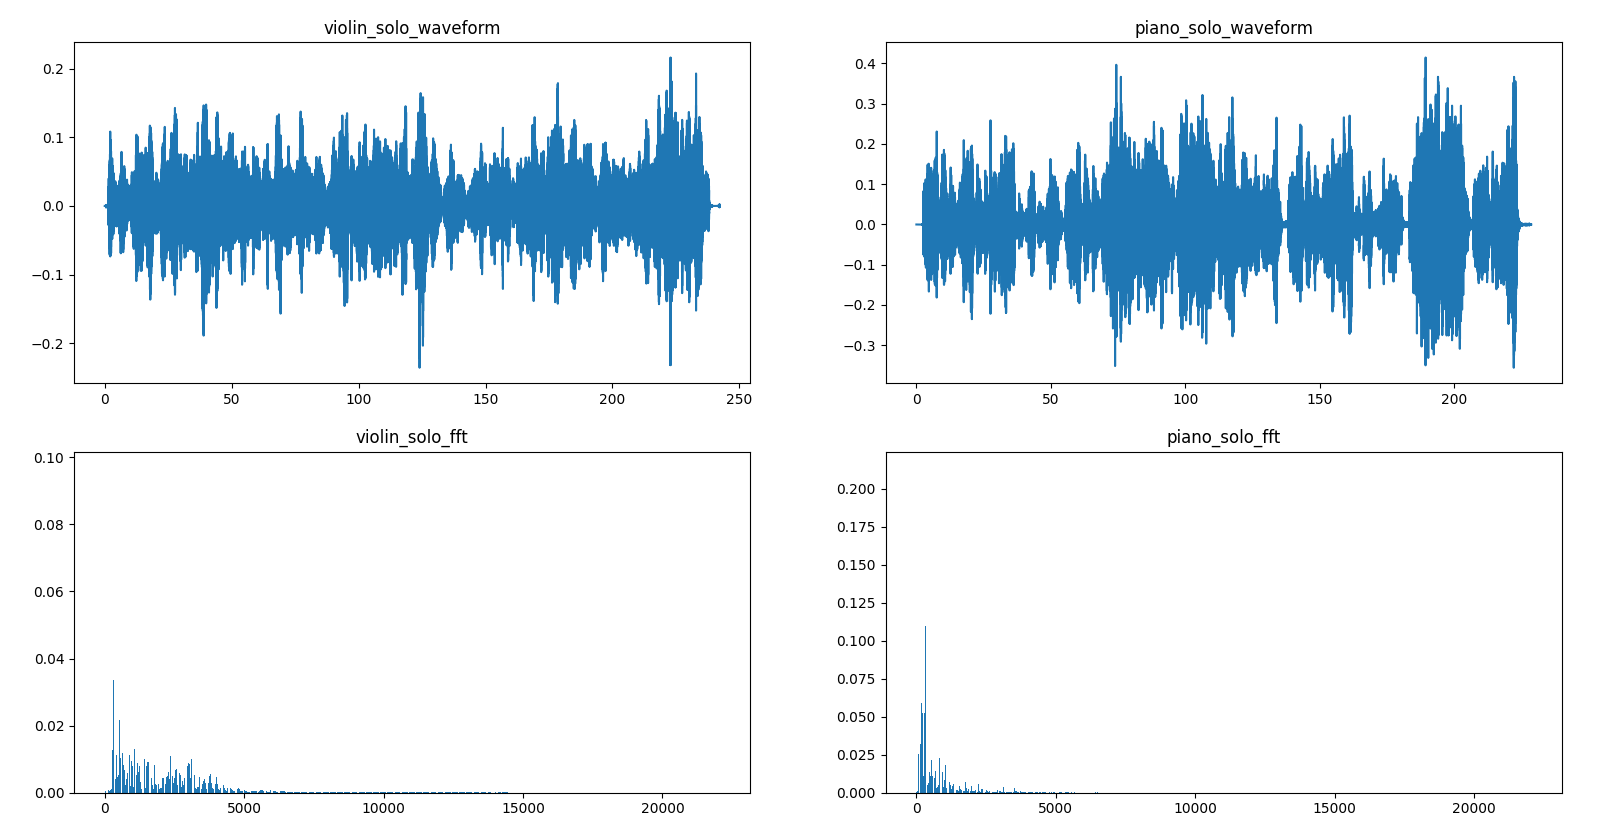
\includegraphics[width=\linewidth]{ch3/fig-bandwidth-estimate.png}
    \caption{兩種資料的波形圖(上)與經過FFT轉換後的$F_{band}$圖(下)}
    \label{fig:fig-ch3-bandwidth-estimate}
\end{figure}

最後我們對$F_{band}$的範圍迭帶計算每個區間的累積振幅值占總和值
的比例$f_{range}/\sum F_{band}$,若超過切割比例閥值$r$,則在此頻率點增加一個切割點。
依照上述的切割比例我們得到兩種樂器的頻帶切割點為 \\
\\
Violin = [400,500,600,700,800,900,1000,1100,1200,1300,1500,1600,1700,1800,\\
1900,2000,2100,2300,2400,2500,2600,2700,2800,2900,3000,3200,3400,3600,3800,\\
4000,4200,4500,4800,5300,5800,6500,7400,8600,10400,13000,18000]\\
\\
Piano = [100,200,300,400,500,600,700,800,900,1000,1100,1200,1300,1400,1500,\\
1600,1700,1800,1900,2000,2100,2200,2300,2400,2500,2600,2700,2800,2900,3000,\\
3200,3400,3600,3900,4100,4400,4800,5300,5900,6900,8700,17300]\\
\\
在訓練BSRNN模型時我們將會套用上面兩個頻帶切割範圍做訓練。

\pagebreak

\section{音樂追蹤模組} \label{ch3-st-music-tracking-module}
此模組是參考~\cite{Lin2020AHumanComputerDuetSystem}的Real-Time Music Tracker來重新實現,
本節將分成兩個部分說明,
\ref{ch3-subst-DTW}節至\ref{ch3-subst-GBA}節
會介紹實現音樂追蹤模組所使用到的演算法並詳細說明改進的部分,
\ref{ch3-subst-data-manager}節至\ref{ch3-subst-decision-maker}
會介紹每個元件的設計與改動。

\subsection{動態時間規整(Dynamic Time Warping, DTW)} \label{ch3-subst-DTW}
DTW~\cite{Sakoe1978Dynamic},
是一種用來計算兩個時間序列資料之間相似度的方法。
給定兩個時間序列
$X = (x_1, x_2, \dots x_N), N \in \mathbb{N}$和
$Y = (y_1, y_2, \dots y_M), M \in \mathbb{M}$,
其中N和M為兩個時間序列的長度,
$x_N$和$y_M$是任兩個具有時間順序且形狀相似的資料,例如音樂、語音等等,
如\cref{fig:fig-ch3-dtw-example}所示。
\begin{figure}[!hbt]
    \centering
    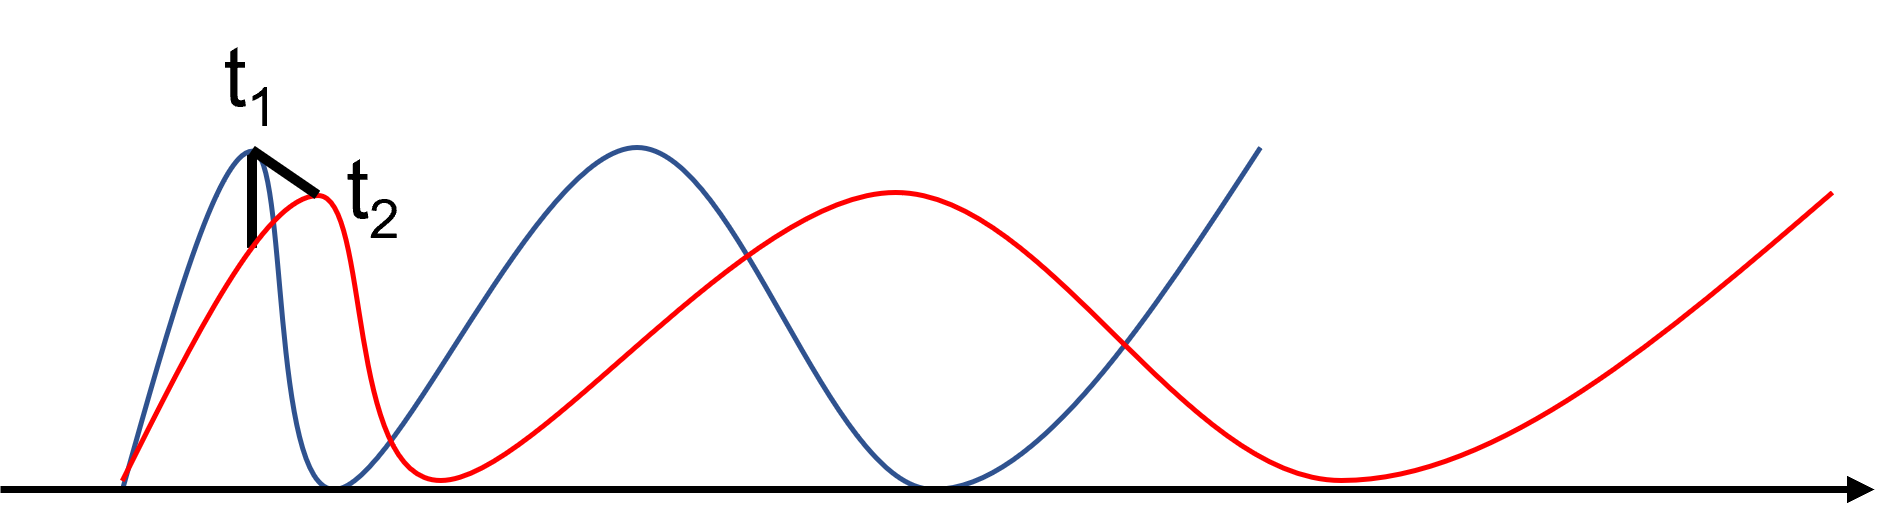
\includegraphics[width=\linewidth]{ch3/fig-dtw-example.png}
    \caption{兩個相似的時間序列:藍色: $X$\ 紅色: $Y$}
    \label{fig:fig-ch3-dtw-example}
\end{figure}

可以看到計算$X[t_1]$與$Y[t_1]$的距離,並不會是相似的資料點,
但若計算$X[t_1]$與$Y[t_2]$的距離,就會被認為是兩個相近的資料點,
因此當兩段相似的資料但在時間軸上並不是對齊的,就適合用DTW演算法動態對齊時間。
考慮到時間序列的長度不一定相等的情況,例如不同人演奏同一個音符可能會有不同的速度差異,
因此DTW通常採用動態規劃的方法來計算相似度。

首先使用歐基里德距離\cref{eq:compute-dtw-cost-function}
計算X與Y所有時間點的距離,
\begin{equation}
    \label{eq:compute-dtw-cost-function}
    d(i, j) = \sqrt{\left\lvert x_i-y_j\right\rvert^{2}}
\end{equation}

並根據\cref{eq:compute-dtw-cost-matrix-function}
使用動態規劃方式建立距離矩陣$D \in \mathbb{R}^{N \times M}$。
\begin{align}
    \label{eq:compute-dtw-cost-matrix-function}
    \left\{
        \begin{array}{l}
            D(0, 0) = d(x_1, y_1)\\
            D(i, 0) = D(i-1, 0)+d(x_i, y_1)\\
            D(0, j) = D(0, j-1)+d(x_1, y_j)\\
            D(i, j) = d(x_i, y_j) + \min \left\{
                \begin{array}{l}
                    D(i, j-1) \\
                    D(i-1, j) \\
                    D(i-1, j-1)
                \end{array}\right\}
        \end{array}
    \right.
\end{align}

在計算最短路徑時,必須遵守三個限制:
\begin{enumerate}
    \item 邊界限制:路徑的開頭與結束必須為$(x_1,y_1)$與$(x_N,y_M)$
    \item 連續性:若路徑的上一個對齊點為$(i, j)$, 
    下一個對齊點只能是$(i+1, j+1), (i+1, j), (i, j+1)$
    \item 單調性:若路徑的上一個對齊點為$(i, j)$,
    下一個對齊點必須為$(i_{next}, j_{next}) \in (i_{next} \geq i, j_{next} \geq j)$
\end{enumerate}
這是為了使回溯的路徑為連續無倒退且整段序列都被包含在輸出裡,確保對齊的一致性。

最後從$D(N, M)$往前回溯至$D(1, 1)$尋找一條最小的累積距離成本路徑,
計算公式如\cref{eq:dtw-backtracking-function}所示,
選擇回溯點時會確認行、列與對角三個方向的距離成本值,並選擇成本最小的點作為回溯點,
\begin{equation} 
    \label{eq:dtw-backtracking-function}
    \begin{cases}
        \text{$(i_{next}, j_{next}) = argmin_{(i-1,j-1),(i-1,j)(i,j-1)}D(i_{next}, j_{next})$} \\
        \text{Stop},\qquad \text{if $(i, j) = (1, 1)$} 
    \end{cases}
\end{equation}

當回溯點走到起始點$(1, 1)$時,將所有回溯點連起來就得到最後對齊路徑$W$,
如示意\cref{fig:fig-ch3-dtw-path-example}所示,右上角為路徑的結束位置$D(N, M)$,
左下角為路徑的開始位置$D(1, 1)$,綠色路徑即為$W$。
\begin{figure}[!hbt]
    \centering
    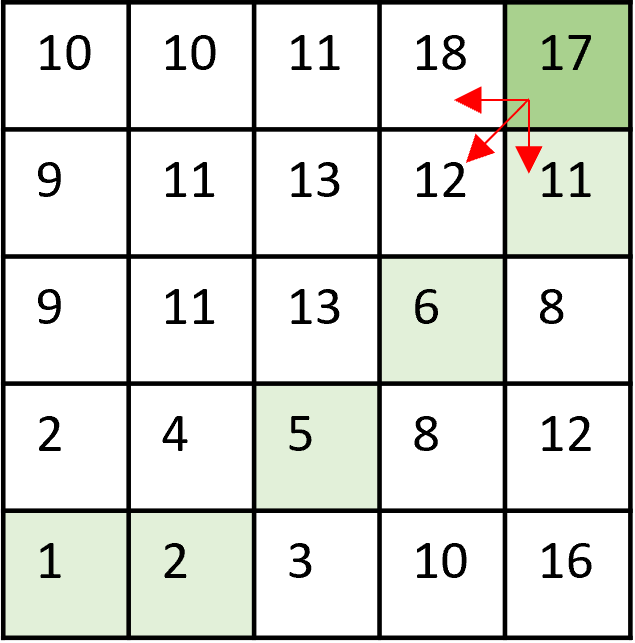
\includegraphics[width=0.4\linewidth, height=0.4\linewidth]{ch3/fig-dtw-path-example.png}
    \caption{DTW 累積距離矩陣回朔路徑示意圖}
    \label{fig:fig-ch3-dtw-path-example}
\end{figure}

本研究所使用的DTW演算法來自python librosa package~\cite{McFee2024librosa}
中的librosa.sequence.dtw函式。

\subsection{線上動態時間規整(Online Dynamic Time Warping, ODTW)} \label{ch3-subst-ODTW}
由於DTW演算法在時間複雜度上為$O(NM)$,屬於複雜度高的演算法,
因此當某個序列的時間較長或是不確定序列的時間長度(例如即時串流音訊)時,
DTW演算法在計算就會花費許多時間。

ODTW~\cite{dixon2005ODTW}由Dixon等人提出,
是基於DTW演算法所做的改良,首先ODTW在計算對齊路徑時並不是回溯計算而是向前增量計算,
並且將計算距離成本的範圍縮小至預先定義的範圍$c$,
因此使ODTW在時間與空間複雜度的表現都是線性$O(N)$,
且因為不需事先知道整個序列的資料,因此適合處理長序列音訊或即時串流音訊。

本研究實現ODTW演算法的步驟如下,
給定兩個時間序列
$X = (x_1, x_2, \dots x_N), N \in \mathbb{N}$和
$Y = (y_1, y_2, \dots y_M), M \in \mathbb{M}$,
其中$X$為現場音訊,因此$N$會隨著串流時間長度而增加,直到串流結束,
$Y$為事先給定的參考音訊,用於對齊現場音訊。
我們想透過距離成本矩陣$D_{total}$找到$X$和$Y$的對齊路徑$W = (W_1, W_2, \dots W_k)$,
其中每個$W_k$為有順序的$(i_k,j_k)$且
$(i,j) \in W$代表兩段序列在$x_i$與$y_j$點上對齊。

距離成本矩陣$D_{total}$透過\ref{ch3-subst-DTW}節所提到的\cref{eq:compute-dtw-cost-function}與
\cref{eq:compute-dtw-cost-matrix-function}計算,另外我們使用$D_{cell}$紀錄單格的距離成本$d$。
我們定義搜尋範圍$c=450$來限制$D_{total}$與$D_{cell}$的大小,
當有新的$i$加入時,我們計算$d(i, j-c), d(i, j-c+1) \dots d(i, j+c)$個點,
此時$j$為目前演算法計算到的參考音訊時間點,而對於$j$點,
則是計算$d(i-c, j), d(i-c+1, j) \dots d(i, j)$,
由於我們無法得知未來的現場音訊,所以只能計算到目前最新的時間點$i$。
上述的計算方式與傳統的ODTW演算法有些微的不同,
在~\cite{dixon2005ODTW}中,每次迭帶時在$(i, j)$方向計算的格數皆為$c$個,
我們將每次迭帶在j方向計算的cell個數改為$2c-1$,
如範例\cref{fig:fig-ch3-odtw-search-range-compute-comparision}所示。
\begin{figure}[H]
    \centering
    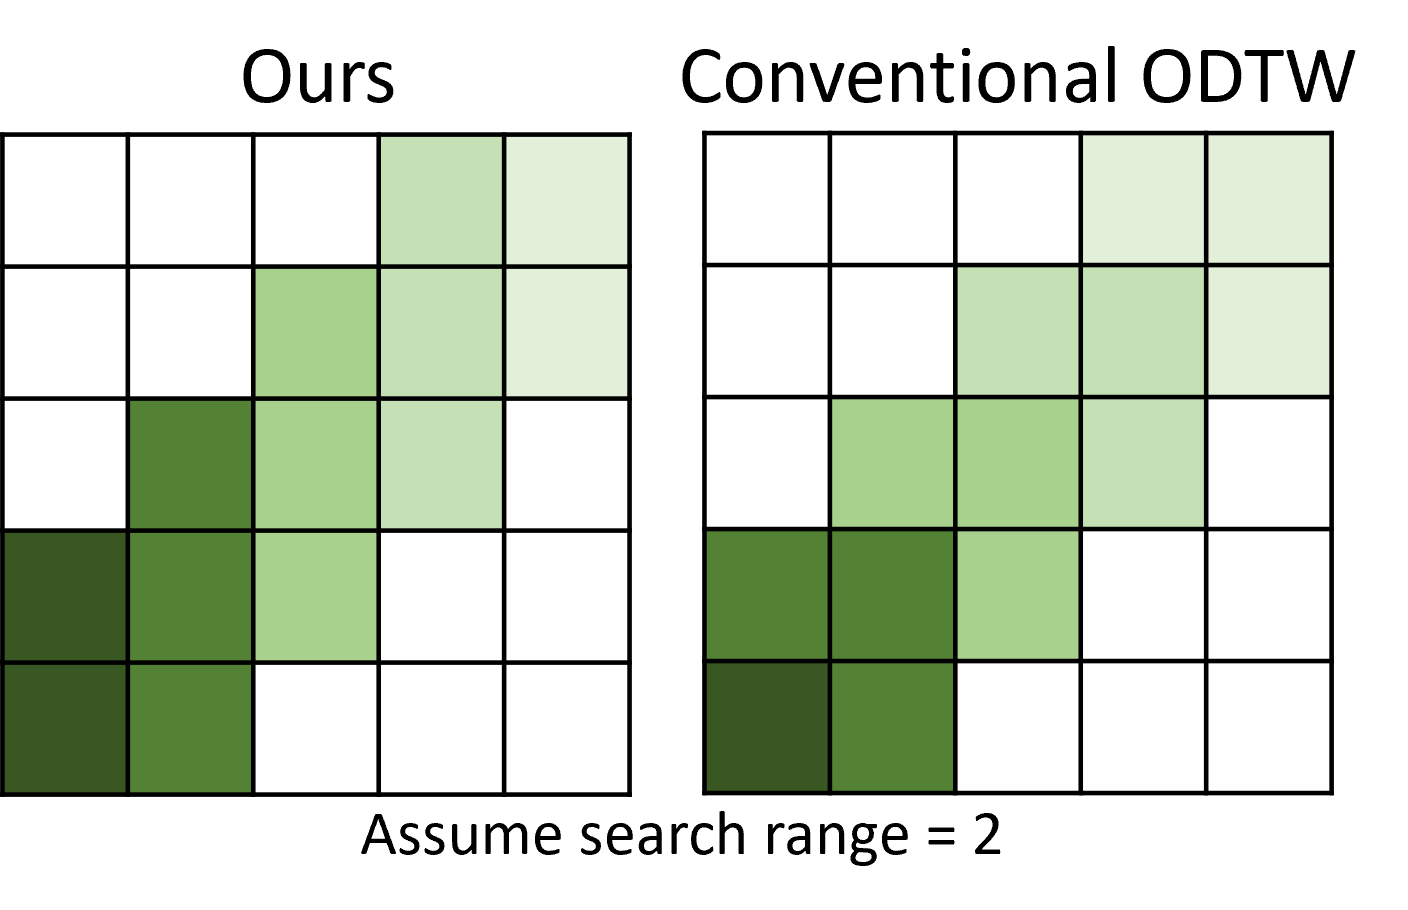
\includegraphics[width=0.7\linewidth]{ch3/fig-odtw-search-range-compute-comparision.png}
    \caption{每個迭帶所計算到的距離成本矩陣格數位置比較}
    \label{fig:fig-ch3-odtw-search-range-compute-comparision}
\end{figure}

會做這樣的更動是因為我們的$i$為現場串流音訊的時間點,
而串流音訊並不會出現相同的時間點(輸出永遠為嚴格單調遞增),
且我們無法得知目前現場音訊的快慢,
因此為了能讓最後輸出對齊位置時有更多的選擇,
我們除了向前計算$(j-c \ \  \text{to} \ \  j)$,
也向後計算$(j \ \  \text{to} \ \  j+c)$參考音訊的距離成本。

在每次計算完最新的$D_{total}$與$D_{cell}$後,
我們使用這兩個成本矩陣計算時間點$i$的對齊位置$output_j$,
首先我們設定兩個參數$L_{upper} = (j+ODTW_{Max\_Run}\times 10)$,
$L_{lower} = (j-1)$,分別代表尋找$output_j$的上下限,
$L_{upper}$的設定為可調的,此數值大約允許現場音訊比參考音訊提前0.6秒,
$ODTW_{Max\_Run}$為參考傳統ODTW演算法的參數,我們將$ODTW_{Max\_Run}$設定為3,
另外考慮到現場音訊並不會突然往前跳回前面的位置,我們的$L_{lower}$不考慮小於$j$的位置。
接著迭帶所有介於$L_{upper}$與$L_{lower}$的點$curr_{j}$,
找到一組點$(i, curr_{j})$的$D_{total}(i, curr_{j})+D_{cell}(i, curr_{j})$值為最小值,
$(i, curr_{j})$即為ODTW的輸出對齊點$(output_i, output_j)$。
另外在計算完目前最小成本值後,為了避免系統一直輸出相同的$output_j$,
當相同的$output_j$輸出次數超過$ODTW_{Max\_Run} \times 3$,我們強制將下一個$output_j$往上加1,
使系統有機會跳脫局部最小值的狀況。

在計算完$(output_i, output_j)$後,
傳統的ODTW演算法會根據目前的$(i, j)$與輸出的$(output_i, output_j)$
決定下一步的走向$(i_{next}, j_{next})$以增加新的距離成本到兩個矩陣中,
走向分別有$(i+1, j+1)$、$(i+1, j)$、$(i, j+1)$三種,
首先當$i < c$時,為了使搜索範圍內的隔數都有計算到距離成本,因此會往$(i+1, j+1)$方向計算,
當$i \geq  c$後,開始根據輸出的位置判斷走向,
當$output_i < i$時,代表目前$i$方向輸出的點較慢,因此往方向$(i+1, j)$計算距離成本;
當$output_j < j$時,代表目前$j$方向輸出的點較慢,因此往方向$(i, j+1)$計算距離成本;
若目前$(output_i, output_j)$皆與$(i, j)$對齊,繼續往$(i+1, j+1)$方向計算新的距離成本。

由於我們的$i$方向為現場音訊的時間點,並不會輸出$i+1$以外的輸出點(嚴格單調遞增),
且我們的輸出$output_j$並不是連續的,使用傳統的方法會可能造成錯誤的對齊,
因此我們將增量對齊的方向改為全部採用$(i+1, j+1)$的方向計算,
但當$i \geq  c$後,我們將目前的$j$設為$output_j$,使系統目前的$j$點保持與輸出相同的位置。

\subsection{貪心向後對齊(Greedy Backward Alignment, GBA)} \label{ch3-subst-GBA}
由於ODTW在對齊時為增量對齊,並不像DTW一樣在計算完兩段音訊的距離成本矩陣後才回溯最佳對齊路徑,
因此通常ODTW的輸出結果會比DTW的輸出結果來的更不穩定。
為了改善上述問題,我們參考~\cite{Arzt2010Towards}中的Greedy Local Search演算法
來設計此方法,此方法配合多執行續的執行可以快速的計算目前位置的向後對齊成本。

給定一個預計輸出位置$(i, j)$作為向後對齊的結尾點,
此位置代表在現場音訊為$i$時,參考音訊估計的對齊位置為$j$,
我們設定一個向後對齊距離參數$GBA_{t}$,
根據現在$i$的時間點與先前輸出位置紀錄$W_{output}$,
我們可以推算出向後對齊的開頭點$(i_{prev}, j_{prev}) = W_{output}[i-GBA_{t}]$。

接著根據距離成本矩陣$D$,我們可以透過\ref{ch3-subst-DTW}節的\cref{eq:dtw-backtracking-function}
計算$(i_{prev}, j_{prev})$到$(i, j)$的對齊成本$W_{cost}$,
在回溯的過程中,因為$(i_{prev}, j_{prev})$與$(i, j)$並不是真正的起始與結束點,
我們設定了最大步數$GBA_{Max\_Run}=3$來限制回溯路徑的走向,
若過程中在行或列的方向走超過$GBA_{Max\_Run}$,
下一步只計算其他兩種方向的對齊成本決定走向。
另外在計算累積距離成本時,我們紀錄回溯路徑的總步數$step_{total}$,
並針對三種走向設計不同大小的值,當走向為對角時,$step_{total}$增加2步,
當走向為行或列時,$step_{total}$增加1步。
這是為了正規化總累積成本,
使每個預計輸出位置在比較累積距離成本時能公平的比較,
最後對齊成本計算公式如\cref{{eq:compute-backtracking-cost-function}}所示。
\begin{equation}
    \label{eq:compute-backtracking-cost-function}
    W_{cost} = \frac{\sum_{w = (i_{prev}, j_{prev})}^{(i, j)}D(w)}{step_{total}} 
\end{equation}

% 解釋為何需要、
% 從候選位置中挑選最好的path、
% 說明參數的設定

% \subsection{即時追蹤系統設計}
% 在音樂追蹤模組中,若無法即時的處理串流音訊導致系統阻塞,就無法達到即時伴奏的效果。
% 因此

\subsection{資料管理者元件(Data Manager Block)} \label{ch3-subst-data-manager}
在線上處理階段啟動前與啟動後,
我們對非串流音訊(參考音訊、伴奏音訊)與串流音訊(現場音訊)
擷取兩種特徵作為其他元件的輸入資料,
分別為高解析度特徵與低解析度特徵,高解析度特徵為梅爾頻譜特徵(Mel Spectrogram),
低解析度特徵為高解析度特徵對時間軸卷積後的重新採樣。
為了管理音訊特徵的處理與傳送,
我們設計了資料管理者來集中管理音樂追蹤模組中所有用到的音訊特徵。

在啟動追蹤系統前,資料管理者會拿到音源分離模組分離出來的參考音訊與伴奏音訊,
對於這兩段完整的音訊,使用44100Hz的取樣率讀取,
並計算短時距傅立葉轉換(Short-time Fourier Transform, STFT)得到頻譜圖,
STFT的參數設定如\cref{table:table-stft-parameter-setting}所示。

\begin{table}[h]
    \centering
    \caption{STFT 參數設定}
    \label{table:table-stft-parameter-setting}
    \begin{tabular}{|c|c|}
        \hline
        \multicolumn{1}{|c|}{Window size} & \multicolumn{1}{|c|}{46ms ($\sim 2029$ frames)}\\
        \hline
        Hop size & 20ms ($\sim 882$ frames)\\
        \hline
        Number of fft & 46ms ($\sim 2029$ frames)\\
        \hline
        Window function & Hanning \\
        \hline
    \end{tabular}
\end{table}

為了使特徵更接近人類的聽覺系統,
我們對STFT頻譜圖做梅爾頻譜分析,得到高解析度特徵。
梅爾頻譜是根據人耳對聲音的敏感度所設計的一種時頻分析方式,
而梅爾頻譜就是由梅爾濾波器組(Mel Filter Bank)與STFT頻譜圖矩陣相乘後得到的結果,
梅爾頻譜圖的參數設定如下\cref{table:table-high-resolution-feature-parameter-setting}所示,
n\_mel為濾波器數量,$f_{min}$與$f_{max}$為使用率波器的頻率範圍,
代表梅爾頻譜特徵在0-8000 Hz使用了84個濾波器將此頻率範圍壓縮成更接近人耳所聽到的樣子。

\begin{table}[h]
    \centering
    \caption{高解析度特徵 參數設定}
    \label{table:table-high-resolution-feature-parameter-setting}
    \begin{tabular}{|c|c|}
        \hline
        \multicolumn{1}{|c|}{n\_mels} & \multicolumn{1}{|c|}{84}\\
        \hline
        Number of fft & 46ms ($\sim 2029$ frames)\\
        \hline
        $f_{min}$ & 0 Hz \\
        \hline
        $f_{max}$ & 8000 Hz \\
        \hline
    \end{tabular}
\end{table}

低解析度特徵由前面所提到的高解析度特徵對時間軸進行卷積,
參數設定如\cref{table:table-low-resolution-feature-parameter-setting}所示,
將每個window size的高解析度特徵窗與window function做卷積
並取平均值代表此低解析度特徵時間點的頻率份量。

\begin{table}[h]
    \centering
    \caption{低解析度特徵 參數設定}
    \label{table:table-low-resolution-feature-parameter-setting}
    \begin{tabular}{|c|c|}
        \hline
        \multicolumn{1}{|c|}{Window size} & \multicolumn{1}{|c|}{600ms ($\sim 30$ frames)}\\
        \hline
        Hop size & 300ms ($\sim 15$ frames)\\
        \hline
        Window function & Hanning \\
        \hline
    \end{tabular}
\end{table}

追蹤系統啟動後,音訊以單聲道、每次傳送與STFT的window size一樣大的樣本至串流音訊到系統,
對於串流音訊的特徵處理方法與上述相同,但由於在處理特徵時我們有設定特徵的window size,
因此必須確保接收到足夠的樣本數才能擷取特徵,否則可能導致特徵蒐集不完全而失真。
因此當系統啟動後,我們將現場音訊記錄下來,當音訊累積足夠的長度時再擷取高/低解析度特徵。
% 由於我們的高解析度特徵的window size大小為46ms,因此會造成系統可能有約46ms的延遲,
% 但在結果的呈現上,並不會影響太多。

\cref{fig:fig-ch3-feature}為現場音訊與參考音訊之特徵圖,
可以看到現場音訊雖然是以frame為單位處理特徵,但將特徵合併後並沒有任何雜訊,
另外可以看到高解析度特徵的時間軸切片較細,低解析度特徵的時間軸切片較粗。

\begin{figure}[!hbt]
    \centering
    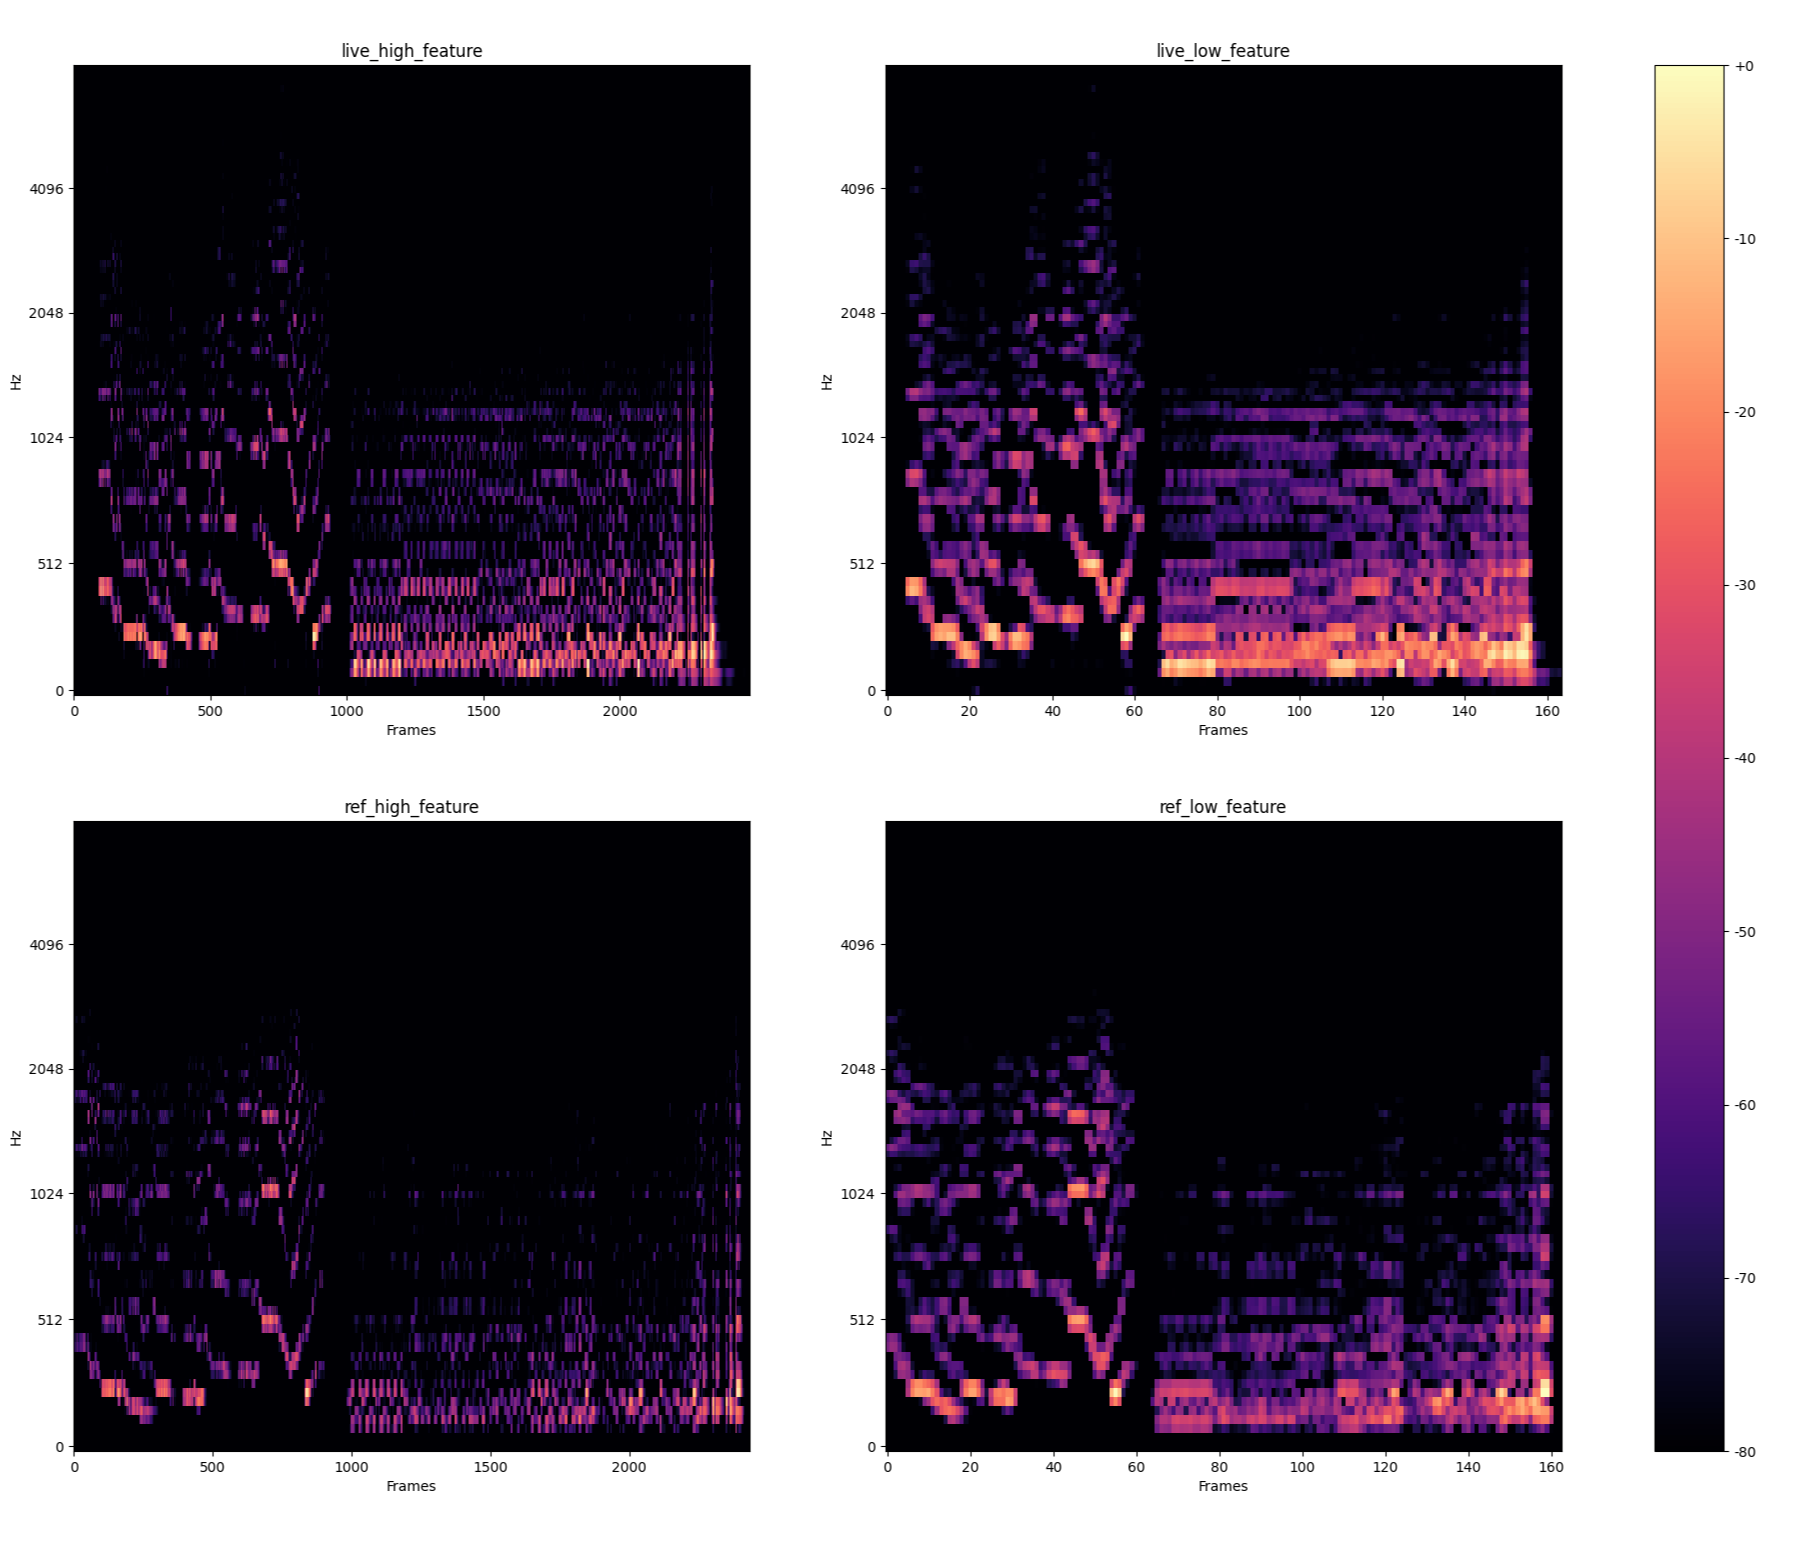
\includegraphics[width=\linewidth]{ch3/fig-feature.png}
    \caption{上:現場音訊的高(左) / 低(右)解析度特徵圖;下:參考音訊的高(左) / 低(右)解析度特徵圖}
    \label{fig:fig-ch3-feature}
\end{figure}

\subsection{音樂偵測器元件(Music Detector Block)} \label{ch3-subst-music-detector}
音樂偵測器為負責偵測使用者開始演奏的時間並觸發後面元件的process,
我們實作了平均振幅的閥值判斷並參考~\cite{Lin2020AHumanComputerDuetSystem}
的DTW對齊成本閥值判斷方法來實現。

當音樂偵測器接收到音訊時,
我們計算平均振幅並根據事先定義的閥值$\theta _{A}$判斷此片段是否為靜音片段,
振幅平均值的計算公式如\cref{eq:avarage-amplitude-function}所示,
$N$為整段音訊的樣本數,$| x[n] \vert$為音訊第n個樣本的絕對值,
A為振幅平均值。
\begin{equation}
    \label{eq:avarage-amplitude-function}
    A = \frac{1}{N} \sum _{n=1}^{N} | x[n] \vert 
\end{equation}
$\theta _{A}$的值是透過統計的方式來決定設定的值,
我們使用已標記音樂開始時間的音訊來一一測試,
已標記的音訊是使用自己錄製的音檔來測試,
我們透過測量每一首的音樂開始時間的振幅值與音樂尚未開始時間的振幅值,
並將音樂開始時間的振幅值加總後取平均獲得,最後我們將$\theta _{A}$設為0.01。

\cref{eq:amplitude-threshold-cases}為平均振幅與閥值的條件判斷公式,
當$A \leq \theta _{A}$時,代表此片段為靜音片段,因此直接回頭計算新的音訊的平均振幅,
當$A > \theta _{A}$時,代表此片段為非靜音片段,可能為音樂開始的地方,
因此將此片段接著使用DTW對齊成本閥值判斷方法。

\begin{equation} 
    \label{eq:amplitude-threshold-cases}
    \begin{cases}
        \text{Compute DTW cost}, & \text{if $A > \theta _{A}$} \\
        \text{Do nothing},  & \text{if $A \leq \theta _{A}$}
    \end{cases}
\end{equation}

DTW對齊成本閥值判斷方法我們參考~\cite{Lin2020AHumanComputerDuetSystem}
,當現場音訊通過平均振幅閥值的判斷後,
我們將音訊擷取為高解析度特徵並與參考音訊開頭0.5秒的高解析度特徵
計算DTW對齊成本${DTW_{cost}}$。
若${DTW_{cost}}$小於設定好的閥值$\theta _{cost}$,
音樂偵測器就會觸發追蹤事件(觸發負責追蹤的processes)。
$\theta _{cost}$的值與上述提到$\theta _{A}$的設定方法一樣為統計的方式,
我們將$\theta _{cost}$設為2000。

\cref{eq:DTW-cost-threshold-cases}為DTW對齊成本與閥值的條件判斷公式,
當$DTW_{cost} \geq \theta _{cost}$時,認定此兩段音訊的相似度不足,
因此不觸發後面的元件並回頭計算新的音訊的平均振幅,
當$DTW_{cost}  < \theta _{cost}$時,認定此兩段音訊具有足夠的相似度被認定為音樂開始的片段,
因此觸發後面的元件並關閉自己的process。
\begin{equation}
    \label{eq:DTW-cost-threshold-cases}
    \begin{cases}
        \text{Trigger tracking event}, & \text{if $DTW_{cost} < \theta _{cost}$} \\
        \text{Do nothing}, & \text{if $DTW_{cost} \geq \theta _{cost}$}
    \end{cases}
\end{equation}

\subsection{粗略位置估計器元件(Rough Position Estimator Block, RPE)} \label{ch3-subst-RPE}
在追蹤系統啟動後,為了避免決策決定者的錯誤對齊,
粗略位置估計器負責使用低解析度特徵計算
目前最新現場音訊幀與參考音訊每一幀的相似度,
並挑出相似度高的前8個粗略估計位置提供給決策決定者參考。

當新的音訊幀經過特徵擷取後,
粗略位置估計器會獲得新的現場低解析度特徵$Live_{low}[t] \in \mathbb{R}^{1 \times F}$,
$t$為最新的低解析度特徵時間點。
此時粗略位置估計器會計算$Live_{low}[t]$與整個參考低解析度特徵$Ref_{low} \in \mathbb{R}^{N \times F}$
的歐基里德距離並紀錄到距離成本矩陣$D_{RPE} \in \mathbb{R}^{t \times N}$,
$N$為$Ref_{low}$的時間長度。
\cref{eq:RPE-Distance-cost-function}
表示在現場與參考的時間點為$[t, n]$時兩個低解析度特徵的距離。
\cref{fig:fig-ch3-RPE-cost-matrix}為實際計算出來的$D_{RPE}$,
越亮的地方代表兩格特徵距離越遠。
\begin{equation}
    \label{eq:RPE-Distance-cost-function}
    D_{RPE}[t, n] = \sum_{f = 0}^{F}\sqrt{
    \left\lvert Ref_{low}[n, f]-Live_{low}[t, f]\right\rvert^{2}} 
\end{equation}

\begin{figure}[H]
    \centering
    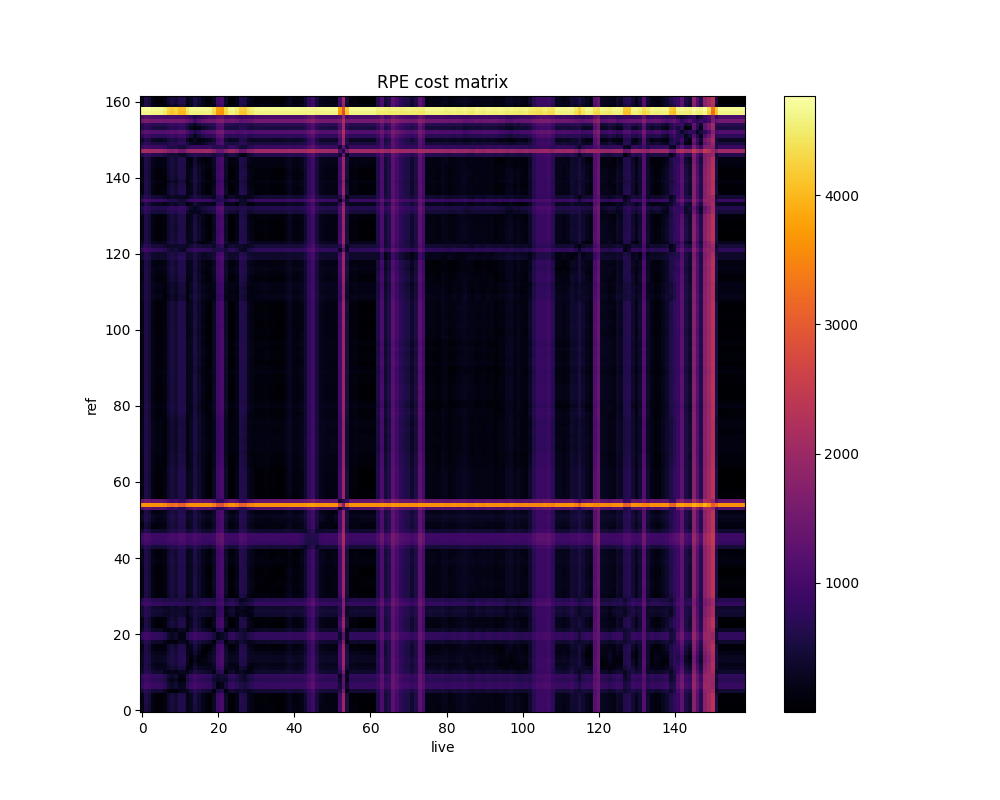
\includegraphics[width=\linewidth]{ch3/fig-RPE-cost-matrix.png}
    \caption{粗略位置估計器的距離矩陣熱力圖}
    \label{fig:fig-ch3-RPE-cost-matrix}
\end{figure}

當$D_{RPE}$累積現場9秒($\sim 30$\ low feature frames)的資訊後,
使用GBA計算時間點$t$時$Ref_{low}$
所有時間點向後對齊9秒的最小路徑成本矩陣$C_{RPE} \in \mathbb{R}^{1 \times N}$,
我們將粗略位置估計器的$GBA_{Max\_Run}$設定為3,
當最小路徑成本值越小,代表此參考點與目前現場位置的相似度越高,
因此我們對$C_{RPE}$做Min-Max資料正規化,公式如\cref{eq:RPE-Min-Max-normalization-function}所示,
所有最小成本路徑值都被正規化到$[0,1]$之間,
並且相似度高的值越接近$1$。
\begin{equation}
    \label{eq:RPE-Min-Max-normalization-function}
    S_{RPE} = 1-\frac{C_{RPE}[n]-min(C_{RPE})}{max(C_{RPE})-min(C_{RPE})},
    n = \left\{0, 1 \ldots N\right\} 
\end{equation}

最後我們獲得相似度矩陣$S_{RPE} \in \mathbb{R}^{1 \times N}$,
為了取出前8個相似度最高的估計位置,
我們對$S_{RPE}$進行降冪排序,並且設定了一個相似度閥值$\theta _{S}$,
當$S_{RPE}$中的值超過$\theta _{S}$且排序在前8個順序時,
才可以做為粗略估計位置輸出給決策決定者,
我們參考~\cite{Arzt2010Towards}的設定,將為$\theta _{S}$設為0.95。
另外累積超過9秒的現場音訊後,
下一次的GBA計算會在1.5秒($\sim 5$\ low feature frames)後,
這是為了節省計算資源,使系統能保持在即時的狀態。
粗略位置估計器的輸出位置點如\cref{fig:fig-ch3-RPE-cost-matrix-with-output}的白色點所示。
\begin{figure}[H]
    \centering
    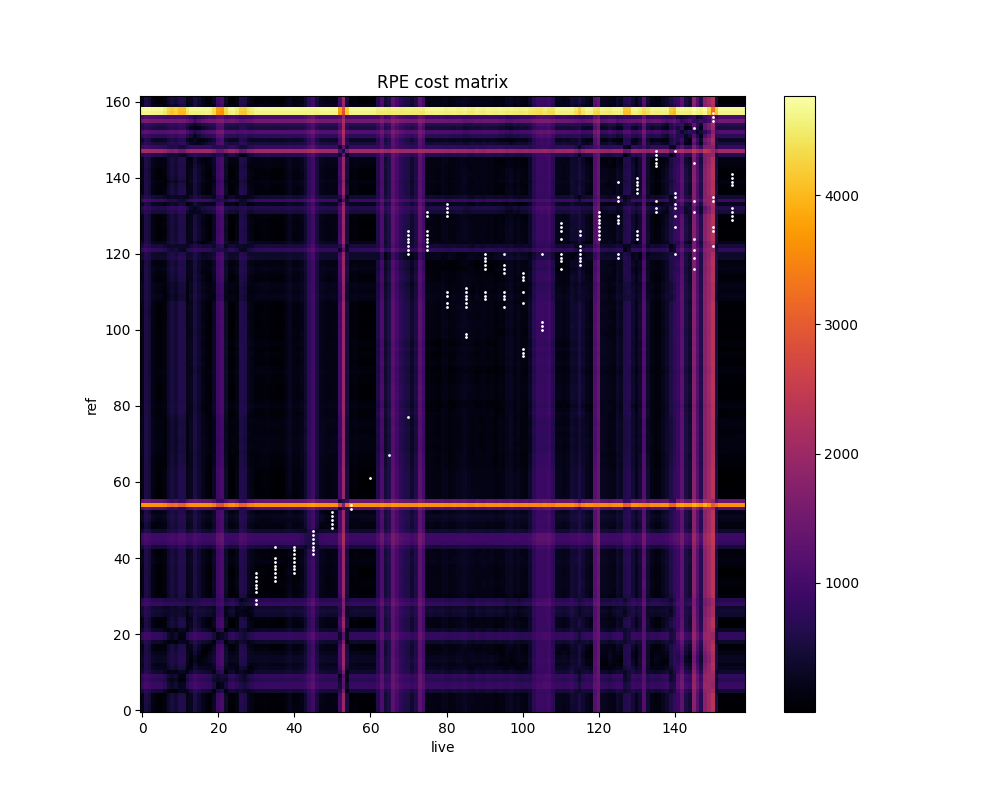
\includegraphics[width=\linewidth]{ch3/fig-RPE-cost-matrix-with-output.png}
    \caption{粗略位置估計器的輸出位置}
    \label{fig:fig-ch3-RPE-cost-matrix-with-output}
\end{figure}

% 使用低解析度特徵、
% 如何計算cost matrix、
% Greedy的設置與做法(在前面解釋)、
% 決定輸出的機制、
% 放圖

\subsection{決策決定者元件(Decision Maker Block)} \label{ch3-subst-decision-maker}
決策決定者由ODTW thread與GBA threads所組成,
負責即時計算現場高解析度特徵與參考高解析度特徵的即時對齊位置,
並參考粗略位置估計器的輸出位置決定最後的輸出點,
為此音樂追蹤模組中最重要的區塊。

在ODTW thread中會持續接收現場高解析度特徵$Live_{high}[t] \in \mathbb{R}^{1 \times F}$
,並與參考高解析度特徵$Ref_{high} \in \mathbb{R}^{N \times F}$
計算兩種距離矩陣$D_{cell} \in \mathbb{R}^{t \times N}$與
$D_{total} \in \mathbb{R}^{t \times N}$,
ODTW的計算方式與參數設定如\ref{ch3-subst-ODTW}節所示,
若目前沒有粗略位置估計器的輸出位置需要加入候選,則輸出ODTW所計算出來的對齊位置。

GBA threads會接收來自粗略位置估計器所計算出來的輸出位置
並使用ODTW的距離成本矩陣$D_{total}$計算GBA結果,
為了不讓粗略位置估計器完全控制輸出結果,
我們將目前ODTW計算出來的輸出位置$output_j$
與$(output_j\pm 15, 30, 45)$一併加入GBA threads計算最終輸出位置。
我們將$GBA_{t}$設為15秒($\sim 750$\ high feature frames),
每個預計輸出位置將會向後計算15秒的最小路徑成本並選出成本最小的位置作為最後輸出。

\cref{fig:fig-ch3-desicion-maker-output}為ODTW的累積距離成本圖與決策決定者的輸出路徑,
我們也將粗略位置估計器的輸出位置(黃色點)結果與ODTW加入預計輸出的位置(桃紅色點)顯示在上面。
為了瞭解決策決定者的輸出路徑是否有偏差,我們將DTW的輸出路徑(淺藍)呈現在
\cref{fig:fig-ch3-offline-and-online-path},並將決策決定者的輸出路徑(綠色)疊加在上面,
可以看到幾乎是與DTW的路徑重疊,代表此系統在即時對齊的能力與DTW離線對齊的能力相當。
\begin{figure}[H]
    \centering
    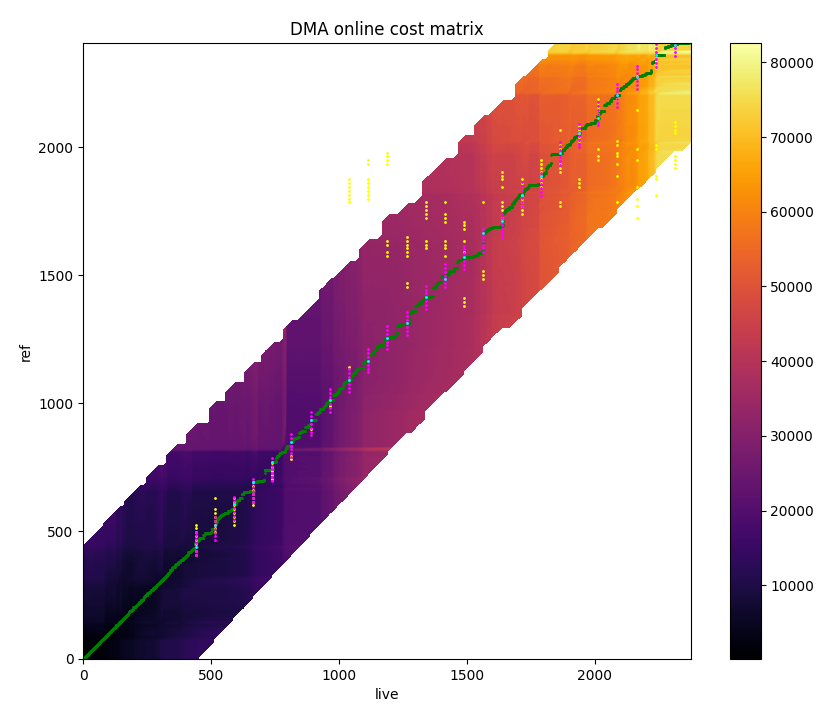
\includegraphics[width=0.8\linewidth]{ch3/fig-desicion-maker-output.png}
    \caption{決策決定者計算的輸出點:\ 淺藍:GBA計算的最後輸出位置\ 綠色:ODTW計算的最後輸出位置}
    \label{fig:fig-ch3-desicion-maker-output}
\end{figure}
\begin{figure}[H]
    \centering
    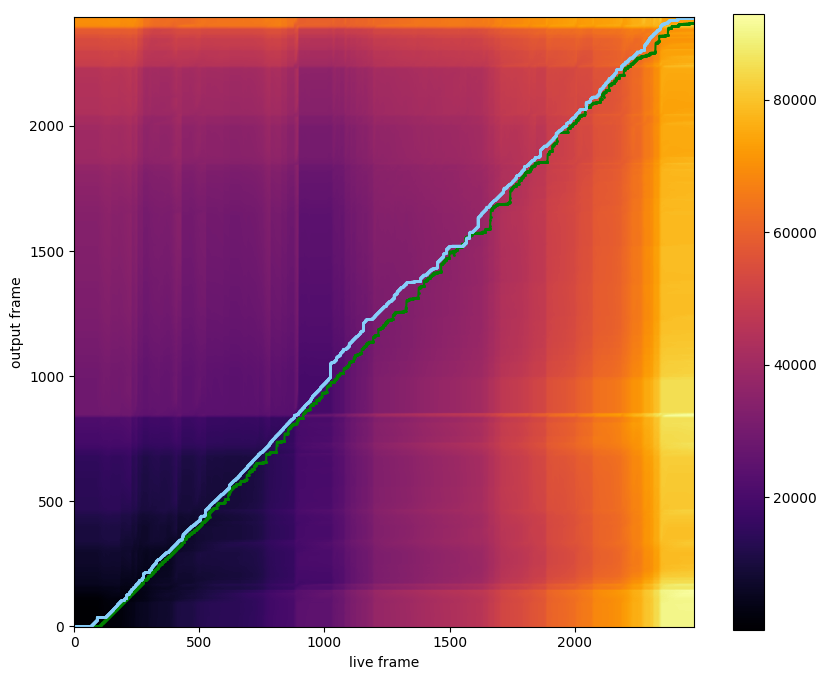
\includegraphics[width=0.8\linewidth]{ch3/fig-offline-and-online-path.png}
    \caption{DTW與音樂追蹤模組的輸出路徑比較圖}
    \label{fig:fig-ch3-offline-and-online-path}
\end{figure}

% 使用高解析度特徵、
% cost matrix的計算
% 清楚解釋ODTW main thread、
% 清楚解釋Greedy threads、
% 清楚解釋輸出的轉換
% 放圖

\pagebreak

\end{document}